\documentclass[../main.tex]{subfiles}

\usepackage{listings}
\usepackage{setspace}

\begin{document}

\chapter*{Chapter 12: Hyperbolic and Parabolic Partial
Differential Equations}

\section*{12.1: EXAMPLES AND CONCEPTS OF HYPERBOLIC PDE'S}

In the last chapter, we discussed in some detail the heat and Laplace's equations,
which are prototypes for parabolic and elliptic PDEs, respectively. We would like
now to introduce some concepts and theory for the wave equation, which is the
prototype for hyperbolic equations. The wave equation models many natural
phenomena, including gas dynamics (in particular, acoustics), vibrating solids and
electromagnetism. It was first studied in the eighteenth century to model vibrations
of strings and columns of air in organ pipes. Several mathematicians contributed
to these initial studies, including Taylor, Euler, and Jean D'Alembert, about whom
we will say more shortly. Subsequently in the nineteenth century, the wave
equation was used to model elasticity as well as sound and light waves, and in the
twentieth century, it has been used in quantum mechanics and relativity and most
recently in such fields as superconductivity and string theory. In general, the
wave equation has a time variable t and any number of space variables JC, y, z,...
and takes the form

\begin{equation}
u_u=c^2 \vartriangle u=c^2(u_{xx}+u_{yy}+...) \label{eq:eps}
\end{equation}

where c is a positive constant and the Laplace operator on the right is with respect
to all of the space variables. Modifications of this equation have been successfully
used to model numerous physical waves and wavelike phenomena. In two space
variables, for example, allowing for a variable wave speed due to depth
differences in an ocean, the PDE:
$u_u=\nabla \cdot[H(x,y,t) \nabla u] + H_u$
has been used to
model large destructive ocean waves. 
\footnote 
{ The symbol $\nabla$, read as "nabla" or "del," is used to represent the gradient operator, which is the
vector of all partial derivatives of a function. Thus for a function of two variables 
$f(x,y)$ , $\nabla f=\nabla  f(x,y)=(f_x(x,y), f_y(x,y))$
. The large dot represents the vector dot product, so in long form: 
$\nabla \cdot [H(x,y,t)\nabla u]= (\partial_x, \partial_y)\cdot (Hu_x, Hu_y)=\partial_x (Hu_x)+\partial(Hu_y)$. In particular, when  $H\equiv 1$ we have $\nabla \cdot [\nabla u]=\partial_x (u_x)+ \partial_y(u_y)=u_{xx}+u_{yy}=\triangle u $, another way to write the Laplacian of u. Such notations
are very common in the literature for partial differential equations involving several space variables.}
In such an application, the function H is the
depth of the ocean at space coordinates (longitude and latitude) (JC, y) and at time /.
The latter term corresponds to the changes in depth due to underwater landslides.
For more on this and other applications of this variable media wave equation, we
mention the text [Lan-99].
\newpage
Much of the general theory of hyperbolic PDEs is well represented by that for the \textbf{one-dimensional wave equation} $(u = u(x,t)$ depends on time / and one space
variable x\ so we proceed now to introduce it through its historical model of a
vibrating string and present some of the theory. At the end of the section we
indicate some differences and similarities of higher-dimensional waves to onedimensional waves. 
\\

We consider a small segment of taut string having length As and uniform tension
T that is acted on by a vertical force q, as shown in Figure 12.1. 
\\

We assume that the string is displaced only in the vertical (transverse) direction,
and let $u(x,t)$ denote the y-coordinate of the string at horizontal coordinate x at the
time t. If we let $\rho$ denote the mass density (mass per unit length) of the string
(assumed constant), then Newton's second law (F = ma) gives us that 
$$-T sin \Theta +T sin (\Theta +\vartriangle \Theta )+q\vartriangle s \rho \triangle su_u (x,t) $$,  
where the first two terms represent the vertical component of the internal elastic
forces acting on the segment of string.

\begin{figure}[H]
	\centering
	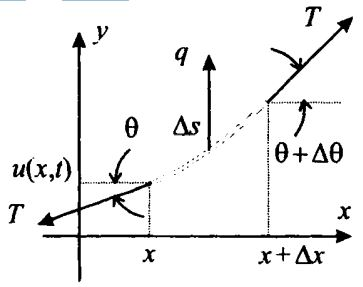
\includegraphics[width=0.4\linewidth]{ch12_1}
	\caption{\textsf{: A segment of a uniformly taut string having tension Tand external load g.
The string is displaced vertically only, and u(x,t) is the vertical level of the string at time /
and horizontal position x .}}
	\label{pfig:ch12_1}
\end{figure}

For small deflections in the string, we have 
$\triangle s\thickapprox \triangle x$
 and also  
 $sin(\theta) \thickapprox \theta \thickapprox u_x (x,t)$
  In the limit as As -» 0, this brings us to

\begin{equation}
Tu_{xx}+q =\rho u_u ,u=u()x,t 
\label{eq:eps}
\end{equation}


which is the \textbf{one-dimensional wave equation with external load term} q. In case
q = 0, this reduces to the one-dimensional wave equation (1) with 
$c=(T/\rho)^{1/2}$
. It turns out that this parameter c is the speed at which the wave (i.e., any solution
of the equation) propagates. This will be made clear shortly. Intuitively, it makes
sense that the speed of any disturbance on a string should increase along with the
tension and decrease for heavier strings. For a derivation of wave equations for
strings under more general hypotheses we refer to the article by S. Antman [Ant80] or Chapter 3 of the textbook by Kevorkian [Kev-00].
\newpage

\begin{wrapfigure}{l}{0.25\textwidth}
    \centering
    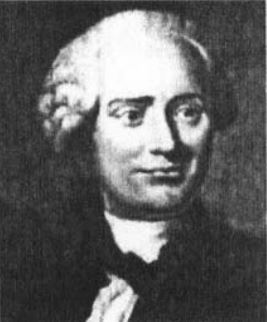
\includegraphics[width=0.25\textwidth]{ch12_2}
   \caption{\textsf{Jean Le Rond
D'Alembert (1717-1783),
French mathematician.}}
   \label{fig:ch12_2}
\end{wrapfigure}


The general solution of the one-dimensional wave
equation was first derived by the French
mathematician Jean D'Alembert. 
\footnote 
{Jean D'Alembert was born in Paris as an illegitimate child of a former nun while the father was out of
the country. Unable to support her son, his mother left him on the steps of a church. The infant was
quickly found and taken to an orphanage. He was baptized as Jean Le Rond, after the name of the
church where he was found. When the infant's father returned to Paris, he arranged for Jean to be
adopted by a married couple, who were friends of his. His adoptive parents brought him up well. He
studied law and earned a law degree. He soon decided that mathematics was his true passion and
studied it on his own. Although mostly self-taught, D'Alembert became an eminent mathematician and
scholar in the same league with the likes of Euler, Laplace, and Lagrange. He made significant
contributions to partial differential equations and his elegant methods, including his solution to the
wave equation, very much impressed Euler. Frederick II (King of Prussia) offered D'Alembert the
presidency of the prestigious Berlin Academy, a position which he declined. He was quite an eloquent
and well-rounded scholar and he made significant contributions to Diderot's famous encyclopedia.
Apparently, D'Alembert was prone to argumentation and his disputes with other contemporary
mathematicians caused him some professional difficulties on several occasions.}
 D'Alemberfs
derivation is simple and elegant and the form of
the solution will give many insights into qualitative
aspects of wave equations. It begins by
introducing the new variables: 

\begin{equation}
\xi=x-ct, \eta=x+ct 
\label{eq:eps}
\end{equation}

We may now think of u as either a function of (x,t)
or of $(\xi,\eta )$. When we use the chain rule to
translate the wave equation (1) into a PDE with
respect to the new variables $(\xi,\eta )$ something
very nice will happen. The resulting PDE will be
extremely easy to solve for the general solution. Applied using (3), the chain rule
gives the following: 

$$u_x = u_\xi \xi_x + u_\eta \eta_x = u_\xi u_\eta$$
\begin{equation}
u_t =u_\xi \xi_t +u_\eta \eta_t =-cu_\xi+cu_\eta
\label{eq:eps}
\end{equation}
\\
\\
\\
In the same fashion, if we differentiate once again, we arrive at
\begin{equation}
u_{xx} =u{\xi \xi}+2u_{\xi \eta}+u_{\eta \eta} , u_u = c^2(u{\xi \xi}-2u_{\xi \eta}+ u_{\eta \eta})  
\label{eq:eps}
\end{equation}
When we substitute equations (5) into the one-dimensional wave equation (1), we
obtain the following version of the wave equation in the new variables $(\xi ,\eta)$ : 

\begin{equation}
u_{\xi \eta}=0.
\label{eq:eps}
\end{equation}
This PDE is very easy to solve, by "integrating" twice. Since it says that $\partial /\partial \eta(u_\xi)=0,$ we can integrate with respect to $\eta$ to get $u_\xi=(F\xi)$,where

\newpage
$F(\xi)$  is an arbitrary function of $\xi$ Next we integrate again, this time with respect
to $\xi$ , to conclude that

\begin{equation}
u(\xi,\eta)=f(\xi)+g(\eta),
\label{eq:eps}
\end{equation}
where $f(\xi)$ and $g(\eta)$ are arbitrary functions of the indicated variables. (Note  $f(\xi)$ is an antiderivative of $F(\xi)$) Translating back to the original variables
using (3) gives us the following general solution of the wave equation:

\begin{equation}
u(x,t)=f(x-ct)+g(x + ct),
\label{eq:eps}
\end{equation}
where $f$ and $g$ are arbitrary functions (with continuous second derivatives). We
point out that each term in (8) represents a wave propagating along the x-axis with
speed c. For example,  $f(x-ct)$  is constant on lines of the form $x = ct$. As time $t$
advances, values of x must also increase to maintain the same value of $f$ (disturbance). Thus the first term represents a wave that propagates in the positive
jc-direction with speed c (right traveling wave). Similarly, the term
$g(x + ct)$ represents a left-traveling wave Both waves travel without distortion
(i.e., the profile of either one of them / units of time later will be the exact same
profile, but shifted to the left or right ct units along the x-axis.)

\begin{figure}[H]
	\centering
	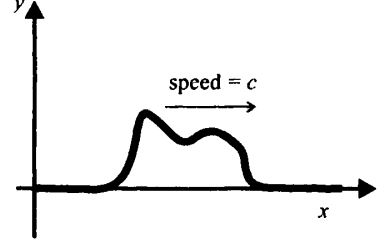
\includegraphics[width=0.4\linewidth]{ch12_3}
	\caption{\textsf{: A right-propagating pulse $f(x - ct$). The general solution (8) of the onedimensional wave equation $u_\eta = c^2 u_{xx}$
also includes a left-propagating pulse. Both
wavefronts propagate without distortion.}}
	\label{pfig:ch12_3}
\end{figure}

D'Alembert went on further with his general solution (8), formulating and
solving a well-posed problem for the one-dimensional wave equation. We
consider a very long string and so consider the one-dimensional wave equation on
the space range $ -\infty <x< \infty$ o, and the time range $ 0 \leqslant t < \infty $ 
Unlike with the heat
equation, it is quite clear from (8) that merely specifying the wave profile W(JC,0) at
time / = 0 is not sufficient to determine a unique solution. Indeed, the initial wave
could come from a single left-moving wave, a single right-moving wave, or more
generally could be made up as a superposition of two waves each moving in
different directions.If we specify both the initial wave profile $u(x,0)$ and its
initial velocity $u_t(x,0)$ ) , then this together with the wave equation will give a well-

\newpage
posed problem. These initial boundary conditions are often referred to as \textbf{Cauchy
boundary conditions}  (or \textbf{Cauchy boundary data}) Thus the \textbf{Cauchy problem
for the wave equation} is summarized as follows: 

\begin{equation}
\left\{\begin{array}{ll}
(PDE) u_\eta=c^2u_{xx}, -\infty<x<\infty, 0<t<\infty, u=u(x,t)\\
(BC's) u(x,0)=\phi(x), u_t(x,0)=v(x)-\infty<x<\infty ,=\leqslant \infty
\end{array} \right.
\label{eq:eps}
\end{equation}
This highlights an important general difference between elliptic PDEs versus
hyperbolic PDEs. Recall from the last chapter that for elliptic PDEs, simply
specifying the value of the solution on the boundary of the domain (Dirichlet
boundary conditions) resulted in a well-posed problem. For hyperbolic PDEs,
more information is needed for the problem to be well posed. We now state
d'Alembert's solution of this Cauchy problem: 
\\
\\
\textbf{THEOREM 12.1:}
(\emph{D 'Alembert 's Solution of the Cauchy Problem?}\footnote
{ In applications, it is convenient to allow functions $\phi(x)$ and $v(x)$ for initial data which may violate
the technical assumptions of having the required derivatives at all values of x. Often there are a finite
set of values (singularities) of x at which either $\phi(x)$ or $v(x)$ may not even be defined or their
derivatives may not exist. Such singularities do not pose any serious problems for d'Alembert's
solution, but they will give rise to corresponding singularities in the solution at all future time values.
See, for example, the initial profile of Figure 12.4 $(\phi(x))$ for a wave problem.  This function has
singularities at the three points where there are sharp corners in the graph $x = -1 , 0, 1$. Future profiles
in the solution shown in Figure 12.5 show also the presence of such singularities. Recall that for
solutions of heat equations that were seen in the last chapter, singularities arising from discontinuities
in an initial temperature distribution or its derivative immediately got smoothed out as time advanced.
This is one of the major distinguishing features between hyperbolic versus parabolic PDE's. In the
former, singularities are preserved and propagate, while in parabolic PDE's, initial singularities
disappear as soon as time becomes positive.} 
Suppose that
the function $\phi(x)$ has a continuous second derivative and $v(x)$ has a continuous
first derivative on the whole real line. Then the Cauchy problem (9) for the onedimensional wave equation has the unique solution given by 

\begin{equation}
u(x,t)=\dfrac{1}{2} \phi(x+ct)+\phi(x-ct)+\dfrac{1}{2c} \int_{x-ct}^{x+ct} v(s)ds
\label{eq:eps}
\end{equation}
Proof: Substitution of the general solution (8) into the BCs of (9) produces (put /
= 0): 
$$\phi(x)=f(x)+g(x), and v(x)=-cf'(x)+cg'(x)$$
Integrating the second equation and dividing by c gives:$(1/c) \int_{0}^{x} V(s)ds=g(x)-f(x)$
(Since $f(x)$ and $g(x)$ are arbitrary functions we can assume that the
constant of integration is zero.) This last equation together with the first of the
original pair are easily solved to give:

$$f(x)=\dfrac{1}{2}[\phi(x)-\dfrac{1}{c}] \int_{0}^{x} V(s)ds] , g(x)=\dfrac{1}{2}[\phi(x)+\dfrac{1}{c}] \int_{0}^{x} V(s)ds]$$
\newpage
Substituting these formulas into (8) now lets us write the solution as: 
$$f(x-ct) + g(x + ct)=\dfrac{1}{2} [\phi(x+ct)+\phi(x-ct)]+\dfrac{1}{2c} [-\int_{0}^{x-ct} v(s)ds+\int_{0}^{x+ct} v(s)ds]'$$
which equals the expression in (10). 
\\

We emphasize that the foregoing analysis was only for one-dimensional waves
on an infinite string. Of course, infinite strings do not exist, but for long strings, or
for modeling disturbances on finite strings for limited time intervals, the above
analysis can lead to useful insights. It is rare to have such an explicit analytical
general solution. Soon we will consider boundary conditions that will require
nonanalytical numerical methods, and finite-difference methods will be employed
as in the last chapter. For now, let us get some hands-on experience with
traveling waves. In the following example, we will get MATLAB to create a
series of snapshots of a solution of a natural wave problem.
\\
\\ 
\textbf{EXAMPLE 12.1:} (A Plucked Infinite String) Consider what happens to a long
string that is plucked with three fingers as shown in Figure 12.4 and then released
(at time $t = 0$). Assume that the units are chosen so that wave speed $c=(T/ \phi)^1/2$ equals 1. Using d'Alembert's solution, get MATLAB to create a series of
snapshots of the wave profiles for each of the seven times starting with time $t = 0$
and advancing to $t = 3$ in increments of 0.5. 
\begin{figure}[H]
	\centering
	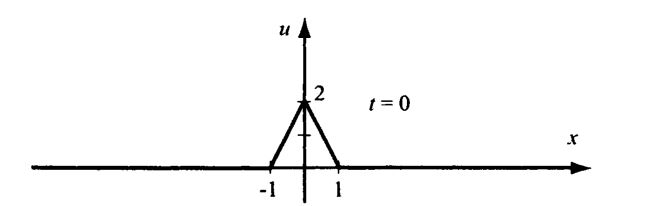
\includegraphics[width=0.6\linewidth]{ch12_4}
	\caption{\textsf{ Initial profile for the plucked string of Example 12.1.}}
	\label{pfig:ch12_4}
\end{figure}

SOLUTION: In the Cauchy problem (9), we put $c = 1$, and $v(x) = 0$ (since at
time $t = 0$, the three-finger plucked string is released with no initial velocity).
From Figure 12.4, we can write the initial profile of the string as

$\phi(x)=
\begin{cases} 2-2\vert x\vert,  for \vert x\vert \leqslant 1\\
0, for  \vert x\vert\geqslant 1
\end{cases}$
It is not too difficult to analyze the resulting wave
[0, for |JC| > 1
propagation analytically using Theorem 12.1, but a MATLAB code can be easily
written to produce snapshots and/or movies of this and more complicated waves.
Since an inline function construction is not appropriate for functions whose
formulas change, we first construct an M-file for the function $\phi(x):$
\newpage
\begin{verbatim}
function y = EX121(x)
if abs(x)<l, y=2-2*abs(x);
else y=0;
end
\end{verbatim}
Using this M-file in the following code, we create relevant vectors to produce the
snapshots, and we use the \textit{subplot} command to conveniently collect all of the
profiles in a single figure. The resulting MATLAB plot window is reproduced in
Figure 12.5. 

\begin{lstlisting}
>> x=-5:.01:5;
>> counter =1;
>> for t=0:.5:3;
		xl=x+t; x2=x-t;
		for i=l:1001
			u(i)=.5*(EX12_l(xl(i))+EX12_l(x2(i)));
		end
		subplot(7,1,counter)
		plot(x,u)
		hold on
		axis ([-5 5 -1 3]) rsWo fix a good axis range.
		counter=counter+l;
	end 
\end{lstlisting}

EXERCISE FOR THE READER 12.1: Following the procedure for making a
movie in Section 7.2, get MATLAB to create a movie of the solution of the wave
problem of Example 12.1 for the time range $0</<4$ . Play it back at varying
speeds (and perhaps with varying repetitions).\\
\\
EXERCISE FOR THE READER 12.2: (a) Write a function M-file:

\begin{verbatim}
function [] = dalembert(c,step, finaltime, phi, nu, range),  
\end{verbatim}
for creating a series of snapshots for the solution of the one-dimensional wave
problem (9). The inputs should be: a positive number c for the wave speed, a
positive number \texttt{step}  for the time steps of the snapshots, and another positive
number \texttt{ finaltime } for the time limit of the snapshots. Also, the initial data of
the problem will be inputted as two inline or M-file functions \textbf{phi} and \texttt{nu} The
last input variable is a 4x1 vector \texttt{range} for the xy-axis range to use in the
snapshots. There will be no output variables, but the program will produce a
graphic of snapshots of the Cauchy problem (9) starting at time t = 0 and
continuing in increments of \texttt{step} until \texttt{ finaltime } e is exceeded.\\
(b) Run your program using the data of Example 12.1.\\
(c) Run your program on the "hammer blow" problem that consists of the Cauchy
problem (9) (for the wave equation) with c = 1, <p(x) = 0, and
$V(x)
\begin{cases} 
1, for \vert x \vert \leqslant 1\\
0, for  \vert x\vert\geqslant 1
\end{cases}$
Create a series of snapshots of the solution from / = 0 to t = 5 in increments of / = 0.5.\\
(d) Use your program to help you estimate the length of time it takes for the
disturbances of the waves of both parts (b) and (c) above to reach an observer at
\newpage
position JC = 10. How do your answers fit in with the previously mentioned fact
that the waves in making up d'Alembert's general solution of the wave equation
travel at speed c (here c = 1)? 
\begin{figure}[H]
	\centering
	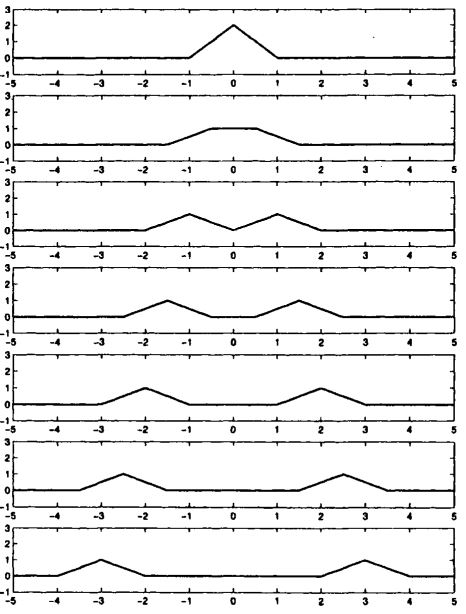
\includegraphics[width=0.6\linewidth]{ch12_5}
	\caption{\textsf{ Progressive snapshots of the solution of the Cauchy problem for the
plucked string of Example 12.1, at times / = 0, / = 0.5, t = 1, ..., t = 3. Note that the initial
disturbance separates into two disturbances that eventually take on the same shape but each
having half the size of the original. The function u(x,t) could also be graphed in three
dimensions as a function of two variables. The snapshots, which are merely "slices** of the
three-dimensional graphs, are often more useful than the latter}}
	\label{pfig:ch12_5}
\end{figure}
We now introduce a concept that will help us to highlight another important
difference between parabolic and hyperbolic PDEs. Note that from d'Alembert's
solution of the wave initial value problem (9), the solution is made up of two
waves propagating at speed c and traveling in opposite directions. The actual
disturbances can travel at speeds less than but not exceeding c (see part (d) of
Exercise for the Reader 12.2). It also follows from d'Alembert's solution that the
value of the solution u of (9) at a certain point (x,t), i.e., the vertical disturbance of
the string at location x and at time t, can only be affected by the initial data
0?,vover the interval $[x-ct,x + ct]$. This interval is called the interval of 
\newpage
 dependence of the "space-time" point (jt,f); and the corresponding triangle (see
Figure 12.6) in the space-time plane is called the \textbf{domain of dependence} of (x, t).
\begin{figure}[H]
	\centering
	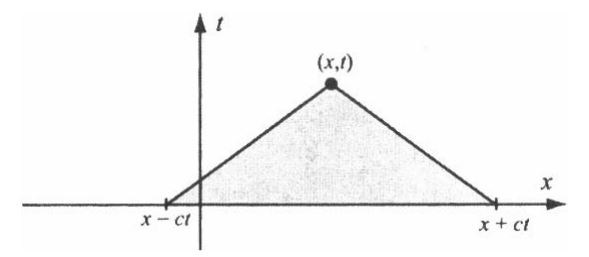
\includegraphics[width=0.6\linewidth]{ch12_6}
	\caption{\textsf{  Illustration of the interval of dependence $[x-ct, x+ct]$ ] (on the x-axis)
for the wave equation on a line. The shaded triangle in the space-time plane (jc/-plane) is
called the domain of dependence. The values of the initial condition functions $\phi(x) and v(x)$ outside of the interval of dependence for $(x,t)$ are irrelevant to the
determination of $u(x,t)$. 
}}
	\label{pfig:ch12_6}
\end{figure}

Although d'Alembert's solution of the wave equation on the infinite string makes
it possible to analyze analytically most of the properties of the solution, the next
variation of a Cauchy problem for the one-dimensional wave equation that we
consider will give rise to analytical formulas that are extremely complicated and
intractable. We now study the wave equation on a string of finite length, which is
fixed at both ends. The precise Cauchy problem that we work with is as follows:
\begin{equation}
V(x)
	\begin{cases} 
(PDE) u_n=c^2 u_{xx}, &  ,0 < x < L, 0< t< \infty ,  u=u(x,t)\\
(BC's)
		\begin{cases}
		u(x,0)=\phi(x), u_t(x,0)=V(x)\\
		u(0,t)=u(L,t)=0
		\end{cases} 
		& ,0 < x < L, 0\leqslant t  < \infty
	\end{cases}
\end{equation}

A model to help visualize this Cauchy problem would be the motion of a guitar
string of length L that is fixed at both ends. What makes a nice analytical formula
impossible here is the fact that once the disturbances reach the ends of the string,
they will bounce back, and things will continue to get more complicated as time
goes on.

Theoretically, we can solve (11) by using d'Alembert's solution for the infinite
string in a clever way. The useful artifice that will be used is called the \textbf{method of
reflections} We first extend the functions $\phi(x) and V(0)$  to be functions on the
whole real line, based on their values in the interval $ 0< x < L$  Labeling these
extensions as $\hat{\phi}(x) and \hat{V}(x)$ ), respectively, they will be created so that they are
odd functions across both of the boundary values $x = 0 and x = L$. Analytically,
this means that
\newpage
\begin{equation}
\hat{\phi}(-x)= -\hat{\phi}(x) ~~~and~~~ \hat{\phi}(2L - x) = -\hat{\phi}(x),~~~ -\infty < x<\infty
\end{equation}
and the corresponding identities for $\hat{V}$ It can be easily verified (Exercise 14)
that the following formula gives such an extension $-\hat{\phi}(x)$ of $\hat{\phi}(x)$.
\footnote{ Technically, this definition does not define
$\hat{\phi}(x)$ for $x=0, \pm L, \pm L, \cdots .$ The original function $\phi(x)$ ) was also not defined at the endpoints x = 0, and x = L. This was only for notational convenience
in the boundary conditions of (11). The boundary conditions corresponding to the ends of the string
being fixed would force   $\phi(0) = \phi(L)$ = 0 so we extend the definition $\hat{\phi}(x)$ to all real numbers by
specifying $\hat{\phi}$ for $\hat{\phi}(0)=\hat{\phi} (\pm L) =\hat{\phi}(\pm L) = \cdots =0.$  The resulting function will be continuous (otherwise the
string would be broken). }

\begin{equation}
\hat{\phi}(x)
	\begin{cases} 
\phi (x)   ~~~ if~~~ 0< x< L\\
-\phi (-x) ~~~ if ~~~ -L < x <0\\
Extend to be periodic of period 2L\\
\end{cases}		
,0 < x < L, 0\leqslant t  < \infty	
\end{equation}
See Figure 12.7 for a graphical depiction of this construction. An analogous
formula is used to construct $\hat{V}(x)$.\\
\\
EXERCISE FOR THE READER 12.3: (Constructing an M-file for a Periodic
Function) (a) For the function $\phi(x) = 1-|1-x|$ on the interval [0, 2] (L = 2).
Write an M-file, called \texttt{y=phihat(x) } that extends the given ftinction to $-\infty < x<\infty$  by the rule of (13). Try to write your M-file so that it does not use
any loops.
\\
(b) Get MATLAB to plot the graph of your \texttt{phihat(x)} on the interval  $-6\leqslant x \leqslant 6$\\

If we solve the corresponding Cauchy problem (9) on the whole real line using as
data the extended functions $\hat{\phi}(x)$ and $\hat{V}(x)$ d v(x) for boundary data, the ftinction $\hat{u}(x,t)$ that arises will, in fact, extend the solution of (11). 


\begin{figure}[H]
	\centering
	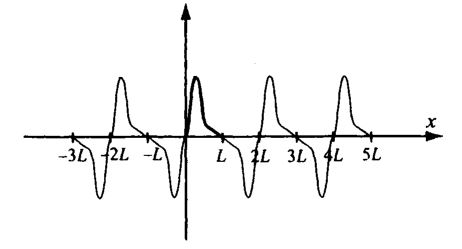
\includegraphics[width=0.6\linewidth]{ch12_7}
	\caption{\textsf{  Illustration of the extension (13) of a function $\phi(x)$ ) defined from x = 0 to x
= L (heavy graph portion) to a ftinction $\hat{\phi}(x)$. that is odd about each of the endpoints x = 0
and x - L }}
	\label{pfig:ch12_7}
\end{figure}
\newpage




\end{document}